企业版WEB是企业版最主要的产品,提供最完整的功能,建议用户使用企业版WEB进行注册为企业版用户。用户在企业版注册会直接生成为企业的交易账号和基金账号,并且创建管理员角色。\par

\noindent{
	注册前需要准备的资料:}\\
	\begin{enumerate}
		\item 管理员手机号码\footnote{建议财务总监或者财务经理}(可以接受短信)
		\item 企业的证件(营业执照、组织机构代码证、税务登记证)
		\item 企业的证件(统一社会信用代码)
		\item 法人的身份证件
		\item 管理员的身份证件信息
		\item 银行开户证明文件
	\end{enumerate}

企业用户注册前请先准备好以上的证件和信息,包括证件的复印件或者扫描件(后续过程需要上传),用户可以访问\href{https://qy.99fund.com/instReg/register.htm}{这里注册}。\par

% 第一步:填写手机号码
\noindent{第1步:填写手机号码并设置登录密码}\\
\begin{figure}[htbp!]
  \centering
  \fbox{
  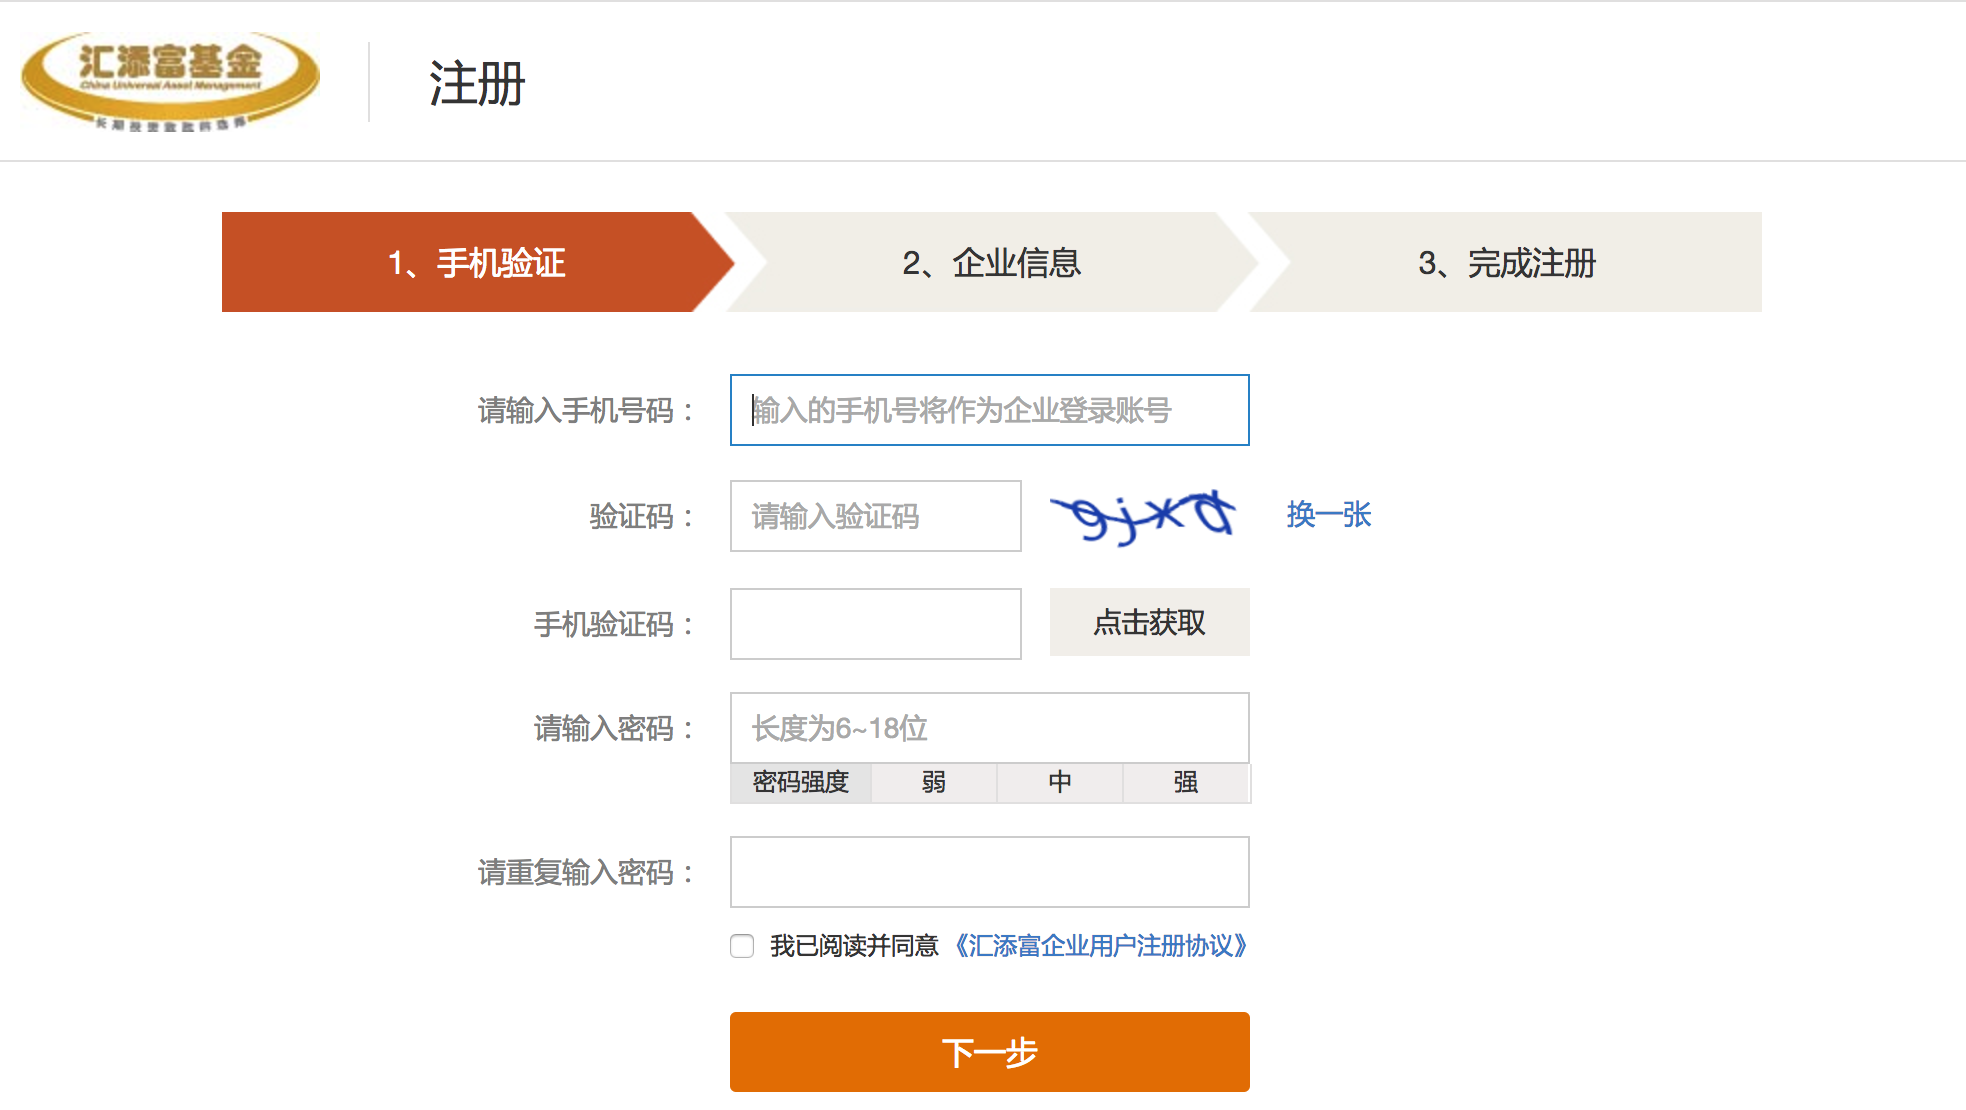
\includegraphics[width=0.9\textwidth]{picture/reg1.png}}
  \caption{填写注册信息}
\end{figure}

% 第二步:填写企业信息
\noindent{第2步:填写企业信息}\\
\begin{figure}[htbp!]
  \centering
  \fbox{
  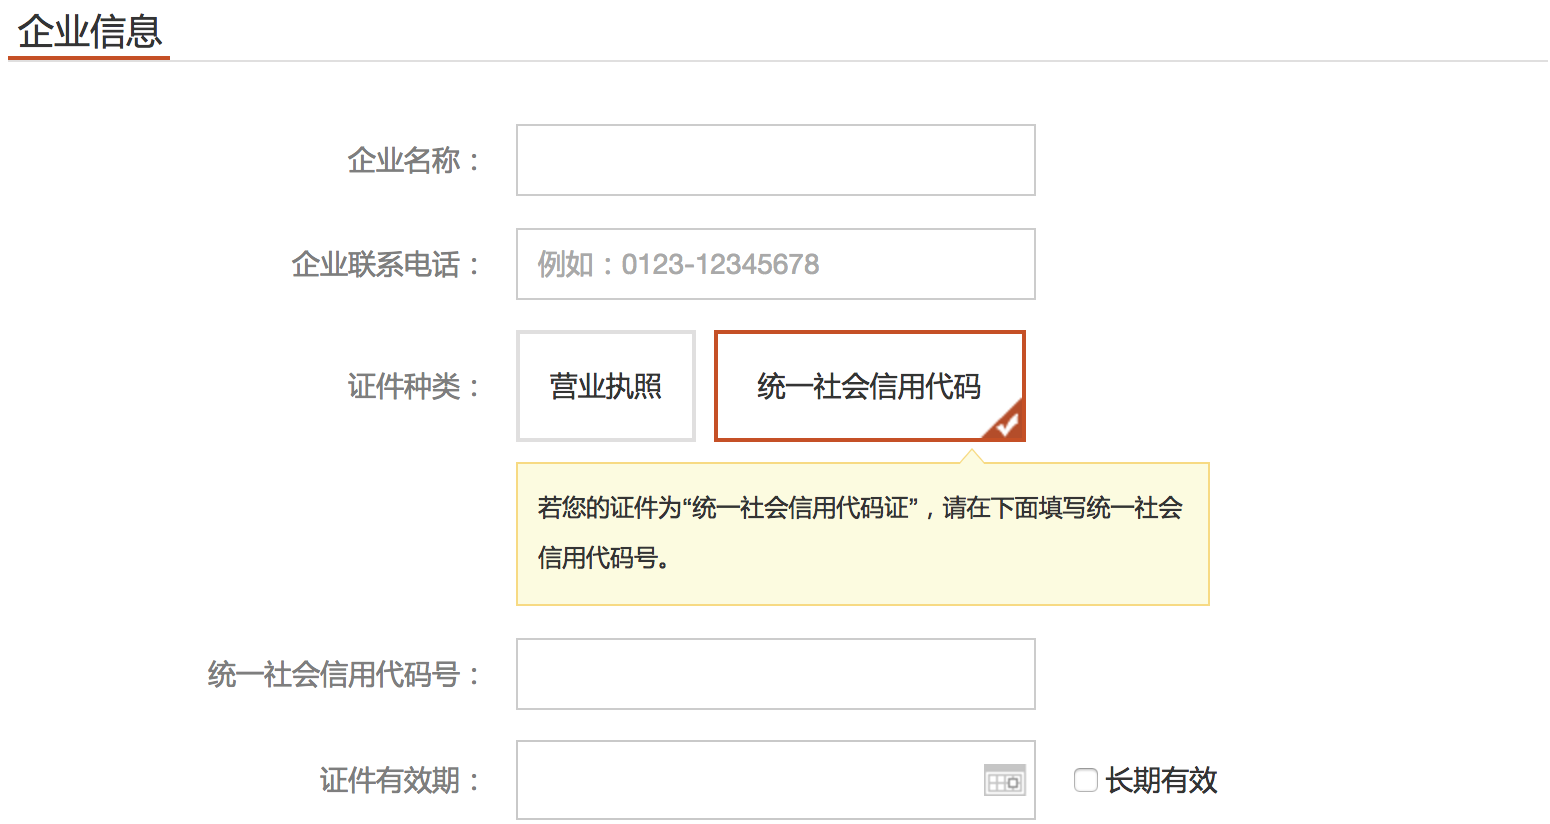
\includegraphics[width=0.9\textwidth,height=6.5cm]{picture/reg2.png}}
  \caption{填写企业信息}
\end{figure}

% 第三步:填写法人信息
\noindent{第3步:填写法人代表信息}\\
\begin{figure}[htbp!]
  \centering
  \fbox{
  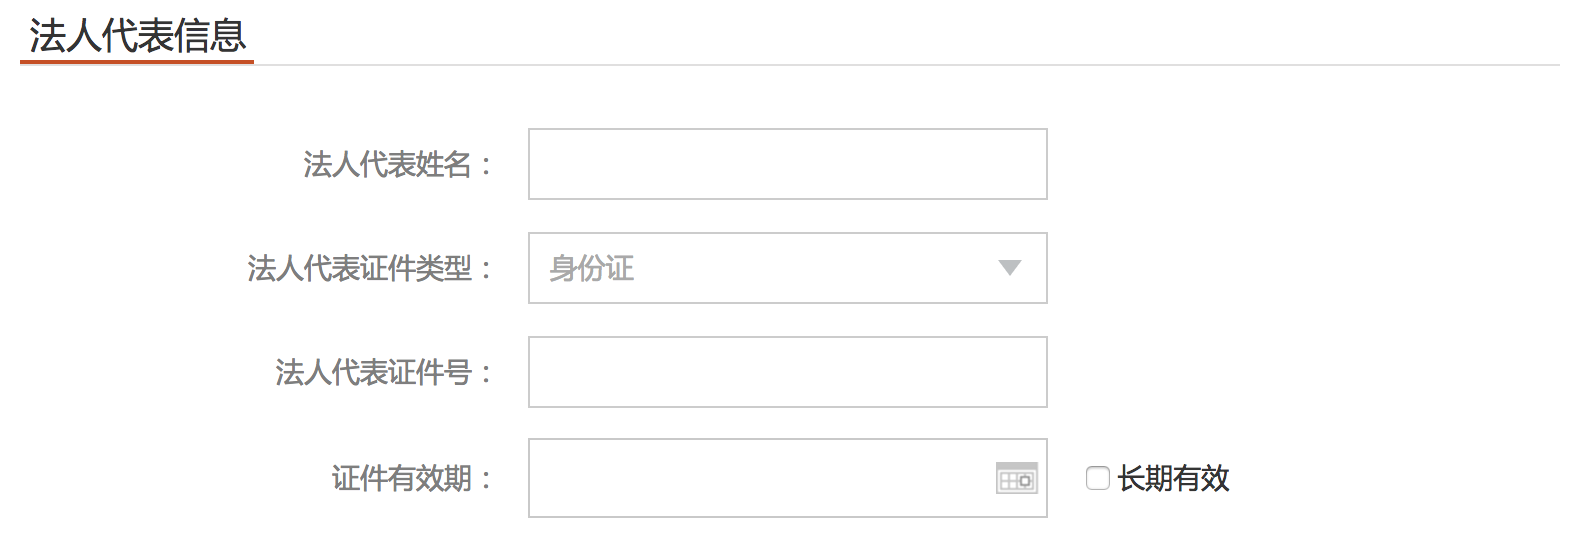
\includegraphics[width=0.9\textwidth]{picture/reg3.png}}
  \caption{填写法人代表信息}
\end{figure}

% 第四步:填写管理员信息
\noindent{第4步:填写管理员信息}\\
\begin{figure}[htbp!]
  \centering
  \fbox{
  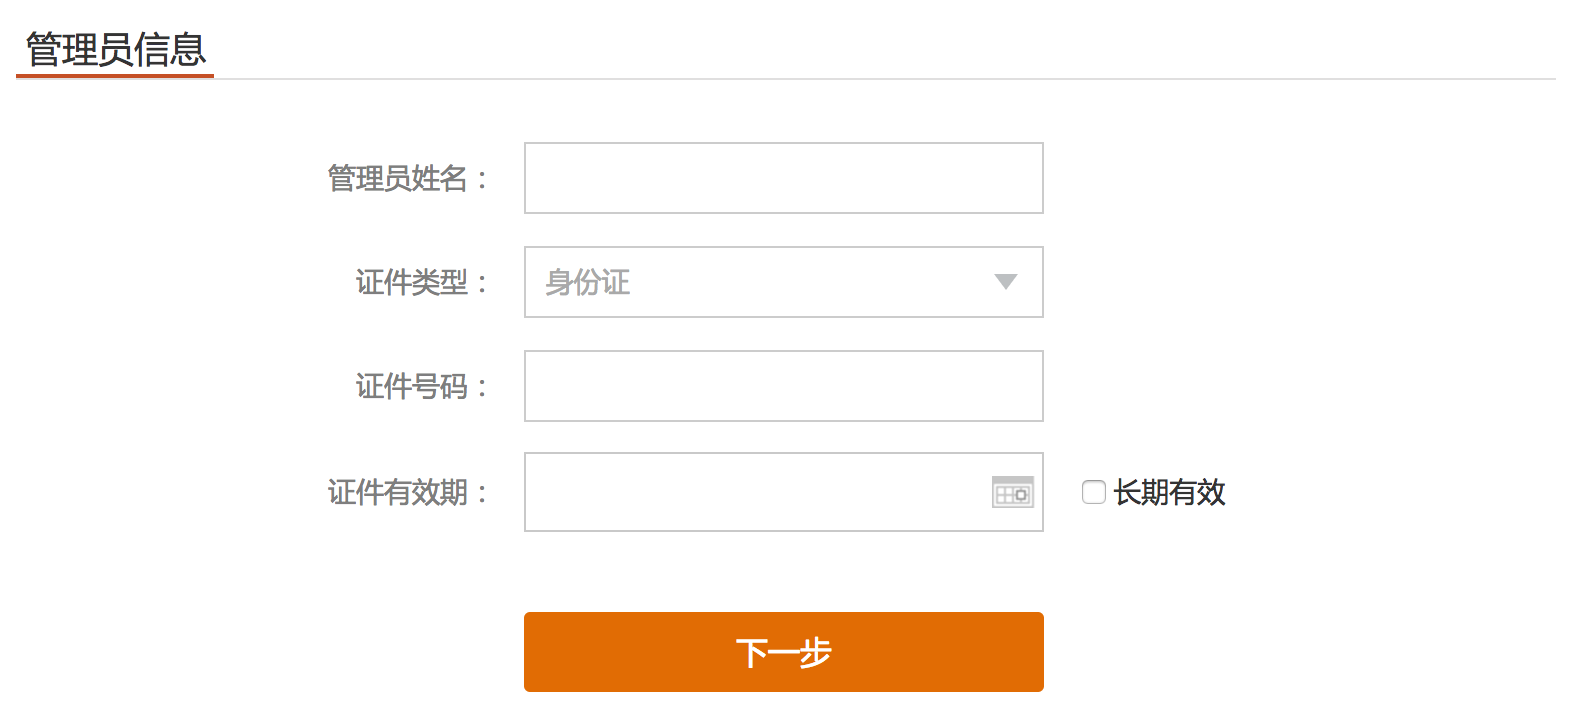
\includegraphics[width=0.9\textwidth]{picture/reg4.png}}
  \caption{填写管理员信息}
\end{figure}

填写完以上信息后,确认无误点击下一步。完成信息的提交,注册的第一阶段完成。这时候在汇添富企业版已经生成企业账户,并根据第1步的手机号码生成管理员账号。\par

% 第五步:注册完成
\noindent{第5步:完成注册}\\
\begin{figure}[htbp!]
  \centering
  \fbox{
  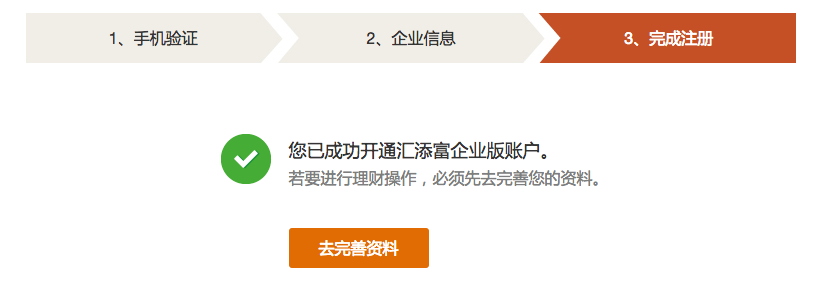
\includegraphics[width=0.9\textwidth]{picture/regs.png}}
  \caption{完成注册}
\end{figure}

\noindent{\large 需要注意的事项:}\\
\begin{enumerate}
	\item 管理员登录密码6-18位
	\item 证件类型为可选:营业执照\&统一社会信用代码
	\item 选择营业执照需要填写其它两个证件号码
	\item 允许一个手机号码注册多个企业账户
	\item 不允许同一证件号码\footnote{指营业执照或者统一社会信用代码,组织机构代码和税务登记证号码同一不影响}注册
	\item 同一证件号码要注册多账户的情况可以通过加后缀实现
  \item 以上第2步至第5步均在一个页面完成
\end{enumerate}
\par
企业版完成注册后,可以使用手机号码(管理员角色)登录企业版,并进一步完成完善资料,参见章节\ref{sec:update_web}。\par
